\begin{frame}
  \frametitle{The Hubble constant}
  \centerline{%
  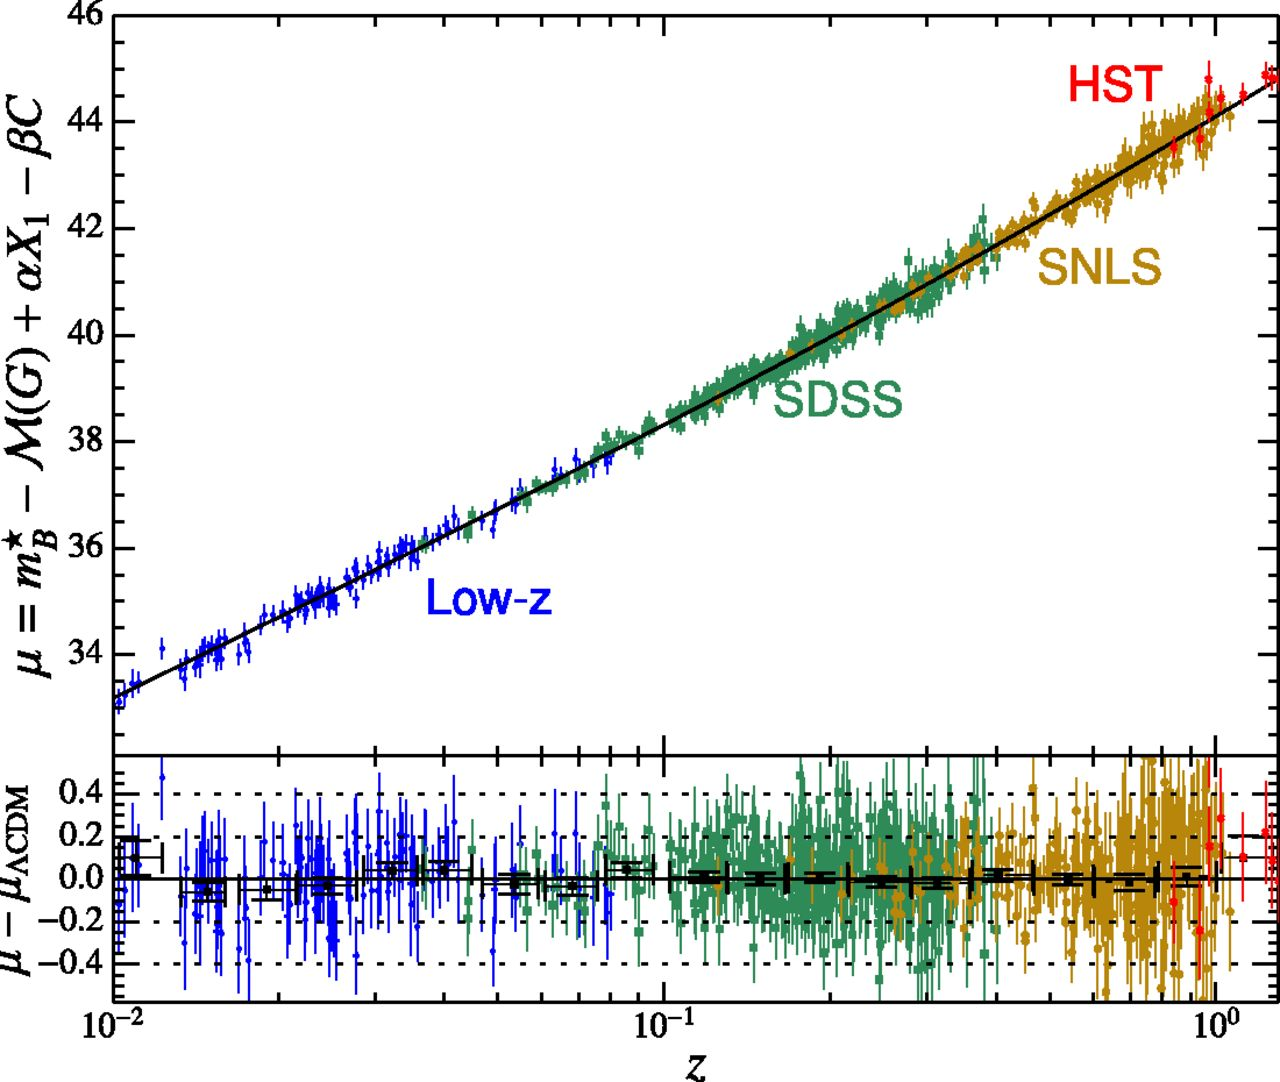
\includegraphics[height=0.8\textheight]{Images/distance_ladder}
  }
\end{frame}

\begin{frame}
  \frametitle{Tension in the Hubble constant}
  \begin{itemize}
      \item<1-> CMB observations:
          \begin{itemize}
              \item<1-> Using our model of the universe + Planck, we find:
              \item<2-> $H_0 = 67.66 \pm 0.42 \mathrm{kms}^{-1} \mathrm{Mpc}^{-1}$
          \end{itemize}
      \item<3-> Supernovae observations:
          \begin{itemize}
              \item<3-> Directly measuring the universe we find
              \item<4-> $H_0 = 73.52 \pm 1.62 \mathrm{kms}^{-1} \mathrm{Mpc}^{-1}$
          \end{itemize}
      \item<5-> Something is wrong with our model of the universe
      \item<6-> Good news!
      \item<7-> Last time this happened, we ``discovered'' dark energy
  \end{itemize}
\end{frame}
